\subsection{Genèse et objectifs du projet symbolist}
\label{subsec:geneseSymbolist}
En qualité de compositeur, Rama Gottfried a été confronté à des problèmes de notation qui ont conduit à l'élaboration du projet \textit{symbolist} de paire avec Jean Bresson.
Rama Gottfried a longtemps utilisé le logiciel \textit{Sibelius}\footnote{\url{https://www.avid.com/fr/sibelius}} pour écrire ses pièces musicales et multimédias. Cependant, la trop grande limitation du logiciel quant à l'écriture d'œuvres contemporaines lui a fait abandonner son utilisation. 
Rama Gottfried opère alors un retour à l'usage du papier pour composer, le support offrant une liberté bien plus importante. Cependant, la numérisation des partitions \og papier \fg engendre une quantité relativement importante de données, représentant un inconvénient certain pour le partage des documents.
En conséquence, Rama Gottfried se tourne vers le logiciel \textit{Adobe Illustrator} pour ses qualités d'application de dessin vectoriel\footnote{\url{https://www.adobe.com/fr/products/illustrator.html}}. \textit{Illustrator} permet au compositeur d'entretenir la relation qu'il avait avec le support papier. L'interface de l'application s'abstrait du cadre de la portée et permet un mode d'expression graphique plus direct. De plus, le plugin \textit{scriptographer} d'\textit{Illustrator} permet à R.Gottfried de créer ses propres outils de dessin \cite{scriptographer2018}. Plus spécifiquement, \textit{scriptographer} permet d'agrémenter la palette d'outils \textit{Illustrator}; un outil est défini par un ensemble de scripts Javascript, qui seront lancés en réponse à des évènements \og souris \fg. Les scripts génèrent des éléments graphiques dans le canevas \textit{Illustrator}. Malheureusement, le plugin \textit{scriptographer} pour \textit{Illustrator} n'est aujourd'hui plus supporté par son équipe de développement. C'est à ce moment là que Rama Gottfried et Jean Bresson ont initié le projet \textit{symbolist}.

\paragraph{Objectifs du projet} \textit{symbolist} propose un environnement pour la notation graphique de pièces musicales et multimédias \cite{gottfried2018}. Bien sûr, les logiciels \textit{wysiwyg} comme \textit{Sibelius} ou \textit{Finale} proposent déjà de noter graphiquement la musique, en utilisant la notation traditionnelle occidentale. C'est sur ce point que ces programmes diffèrent.
Le premier objectif de \textit{symbolist} est de se rapprocher de la composition sur feuille blanche, aussi le compositeur ne se voit imposer aucun système de notation. L'utilisation de la \gls{portee} n'est, par exemple, plus obligatoire.
L'impossibilité de standardiser la notation des œuvres contemporaines a fait privilégier aux créateurs de \textit{symbolist} l'aspect de libre création graphique plutôt que d'imposition d'un canevas notationnel.
Aussi, \textit{symbolist} propose des outils de dessins standards (lignes, formes géométriques...) pour la création de symboles, et permet à l'utilisateur de stocker les symboles créés dans une palette pour réutilisation.
Même si l'interface graphique se détache de la portée, l'idée d'ordonnancer temporellement les symboles créés est conservée. En effet, dans \textit{symbolist}, chaque symbole peut être associé à un symbole de type \textit{staff} (une voix de la portée, en anglais) qui fait office de référence temporelle. Ainsi, les symboles associés à un \textit{staff} se voient attribuer un marqueur de temps selon leur position sur l'axe horizontal. Dans une partition \textit{symbolist}, il est admis que l'axe horizontal représente le temps, même si un symbole n'est marqué temporellement qu'après avoir été associé à un \textit{staff}. En revanche, et contrairement à la portée, l'axe vertical ne représente pas systématiquement la hauteur des sons. Un symbole placé au-dessus d'un autre ne doit pas être interprété comme produisant un son plus aigu. La sémantique de l'axe vertical est laissé à la discrétion du compositeur.

Un autre objectif de \textit{symbolist} est de tirer des symboles graphiques une information interprétable par la machine, qui permettrait de contrôler les paramètres d'une pièce musicale ou multimédia. Inversement, \textit{symbolist} peut être vu comme un transcripteur symbolique des variations des paramètres d'une pièce, recevant de l'information depuis des processus extérieurs et transformant cette information en symboles dans la partition.   
Pour ce faire, et en s'inspirant du format SVG qui décrit des formes graphiques en syntaxe XML \cite{svg2011}, chaque symbole d'une partition \textit{symbolist} est définit par un bundle OSC \cite{wright2002}. Comme présenté dans l'étude bibliographique, un bundle OSC est un ensemble de messages OSC, couples clé-valeur où la clé est exprimée sous forme d'url.
Le listing \ref{lst:bundleOSCMin} présente le bundle OSC minimal décrivant les informations partagées par l'ensemble des symboles d'une partition.

\begin{lstlisting}[language=java, 
				   caption={Messages OSC \'{e}l\'{e}mentaires pour les symboles d'une partition \textit{symbolist}}, 
				   label={lst:bundleOSCMin}, 
				   captionpos={b}, 
				   numbers=none]
/type  "circle"
/name  "myCircle"
/id    "circle/1"
/staff "staff/0"
/w     30
/h     30
/x     150
/y     160 
\end{lstlisting}

Le bundle OSC présenté dans le listing \ref{lst:bundleOSCMin} décrit un cercle nommé \textit{myCircle}, dont l'identifiant est \textit{circle/1}. Le cercle est attaché à un \textit{staff} (référent temporel) dont l'identifiant est \textit{staff/0}. Graphiquement, la figure est définie dans un boîte de largeur 30 pixels et de hauteur 30 pixels. Le centre de la boîte est situé aux coordonnées $(150, 160)$.
L'avantage de décrire les symboles sous forme de bundle OSC réside dans le caractère standard du protocole, permettant de fait l'envoi/réception de données structurées à/depuis un autre programme. Les possibilités d'interfaçage du logiciel \textit{symbolist} s'en voient décuplées.
Dans une optique d'interaction avec d'autres programmes, l'application a pour finalité d'être déployer en tant qu'objet \textit{Max} \cite{puckette1991} et \textit{OpenMusic} \cite{agon1998}, deux langages de programmation visuelle pour l'informatique musicale.  

\subsection{Analyse de l'existant}
\label{subsec:analyseSymbolist}
        
   Au début de ce stage, le logiciel \textit{symbolist} en est déjà à un état de développement avancé. Cette section détaille l'état de l'application d'un point de vue fonctionnel, technologique et architectural, tel qu'il se trouvait au début de la période de formation.

Au commencement du stage, l'interface graphique de \textit{symbolist} offre déjà les fonctionnalités basiques de dessin sur l'espace de la partition. Les différentes vues composants l'éditeur graphique de \textit{symbolist} sont présentées en figure \ref{fig:symbolistUIBefore}.

\begin{figure}[H]
	\centering
	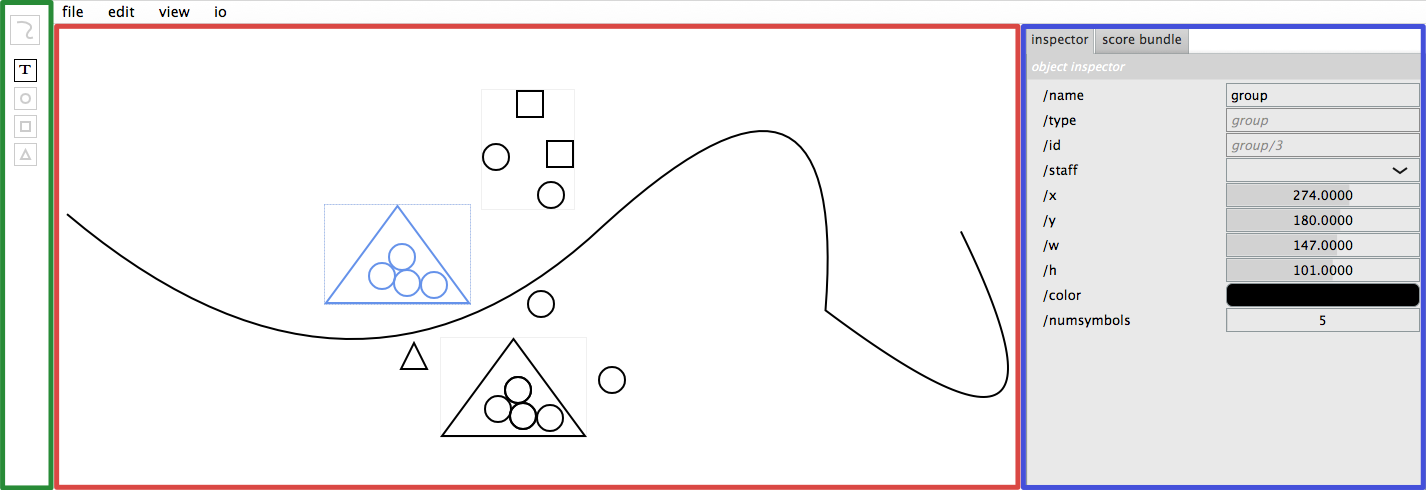
\includegraphics[keepaspectratio=true, width=\textwidth]{SymbolistOutilDeRecherche/i/symbolistUIBefore.png}
	\caption{Éditeur graphique de \textit{symbolist}}
	\label{fig:symbolistUIBefore}
	\small
	\it
	En \textcolor{green}{vert}, la palette des symboles disponibles et dessinables sur la partition. En \textcolor{red}{rouge}, la partition, ou l'espace de composition et d'édition des symboles. En \textcolor{blue}{bleu}, l'inspecteur de symboles, qui présente le bundle OSC associé au symbole graphique couramment sélectionné (symbole surligné en bleu dans la partition).
\end{figure}

L'éditeur graphique de \textit{symbolist} permet à l'utilisateur de dessiner directement sur la partition à l'aide de la souris, dans une modèle d'interaction \textit{wysiwyg} (\textit{what you see is what you get}). Dans \textit{symbolist}, la partition fait référence à l'espace graphique où les symboles sont placés et édités par l'utilisateur. De manière sous-jacente, la partition est stockée comme une liste de symboles. Les symboles de la partition qui sont attachés à un référent temporel, un \textit{staff}, se voient attribuer une valeur temporelle de départ et de fin correspondant à leur point de départ et de fin sur l'axe horizontal. Ces symboles sont ordonnancés temporellement dans la liste reflétant la partition.

De plus, l'éditeur graphique n'est pas le seul moyen d'interagir avec le logiciel \textit{symbolist}. En effet, \textit{symbolist} est également déployer dans une version \textit{objet} pour l'environnement \textit{Max} et l'environnement \textit{OpenMusic}. Dans ces environnements, l'application \textit{symbolist} est représentée comme une boîte, recevant et envoyant des messages à d'autres objets. Les différents messages auxquels répond l'objet \textit{symbolist} dans l'environnement Max sont présentés en figure \ref{fig:symbolistMaxObject}.

\begin{figure}[H]
	\centering
	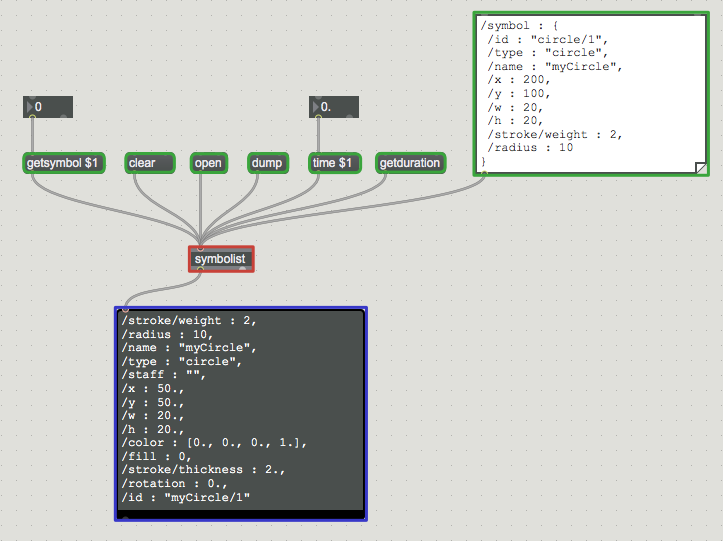
\includegraphics[keepaspectratio=true, width=0.8\textwidth]{SymbolistOutilDeRecherche/i/symbolistMaxObject.png}
	\caption{L'objet \textit{symbolist} dans Max}
	\label{fig:symbolistMaxObject}
	\small
	\it
	En \textcolor{red}{rouge}, l'objet \emph{symbolist} représenté, comme tous les objets \emph{Max}, sous forme de boîte. En \textcolor{green}{vert}, les messages pouvant être envoyés à l'objet \emph{symbolist}.
	En \textcolor{blue}{bleu}, un afficheur de bundle OSC, proposé par une librairie indépendante, témoin des messages de sortie générés par l'objet \emph{symbolist}.  
\end{figure}

Les messages\footnote{Dans Max, un message peut être envoyé à un objet via l'objet \textit{message}, qui n'est autre qu'un bouton cliquable avec un label, à connecter à l'entrée d'un receveur.} compris par l'objet \textit{symbolist} permettent de lire et d'écrire des symboles dans la partition.
Comme exemples de messages de lecture, \lstinline|getsymbol n|, lit le \textit{n-ième} symbole de la partition, \lstinline|time t|, lit le contenu de la partition au temps \textit{t}…
Le résultat de la lecture est envoyé sur la sortie de l'objet \textit{symbolist}.

L'écriture de symboles dans la partition se fait par l'envoi de bundles OSC en entrée de l'objet \textit{symbolist} (voir la figure \ref{fig:symbolistMaxObject}, en haut à droite). 
Enfin, l'éditeur graphique peut être lancé par l'envoi du message \lstinline|open|.

\textit{symbolist} est également déployé dans une version objet \textit{OpenMusic}. La figure \ref{fig:symbolistOMObject} montre un exemple de computation de partition avec l'objet \textit{symbolist} (nommé \textit{sym-score}) dans \textit{OpenMusic}.

\begin{figure}[H]
	\centering
	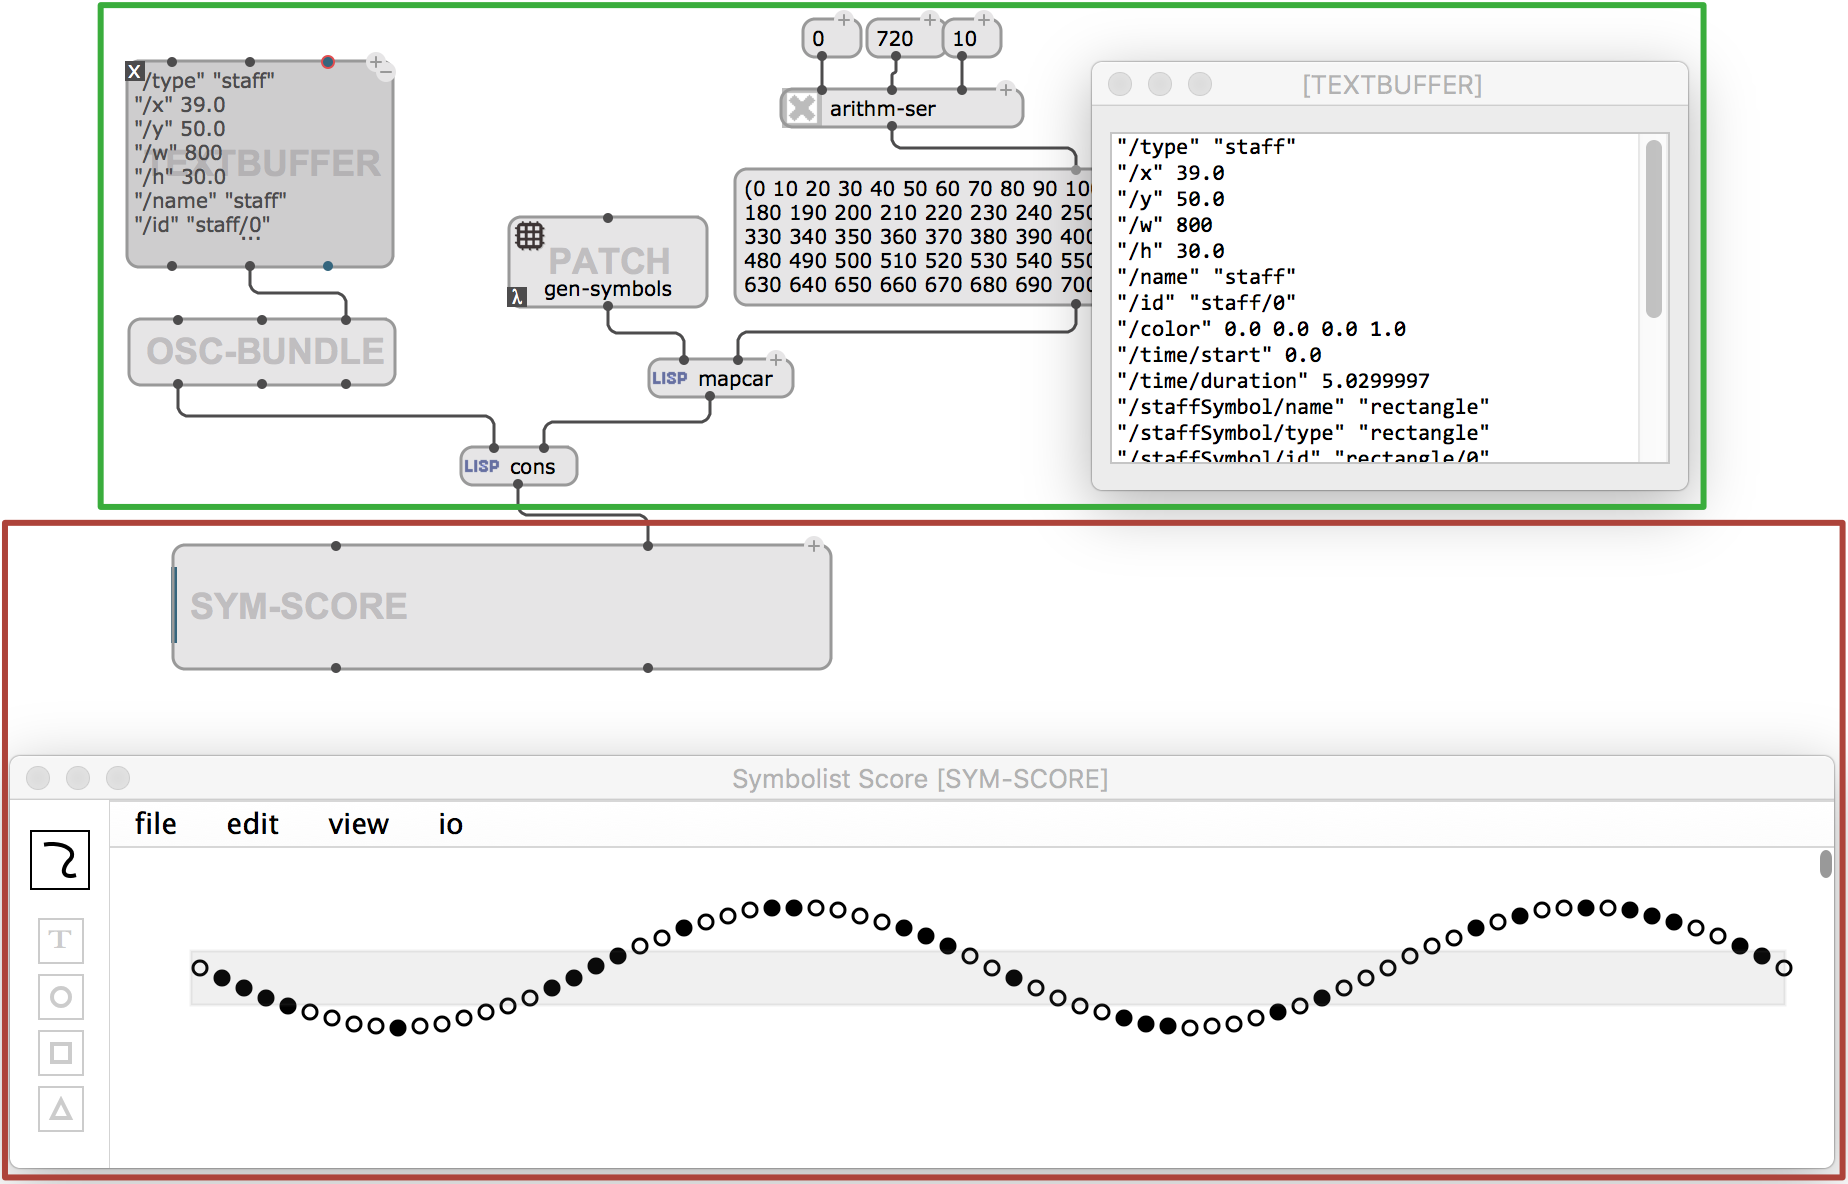
\includegraphics[keepaspectratio=true, width=\textwidth]{SymbolistOutilDeRecherche/i/symbolistOMObject.png}
	\caption{L'objet \textit{symbolist} dans OpenMusic}
	\label{fig:symbolistOMObject}
	\small
	\it
	En \textcolor{red}{rouge}, l'objet \emph{symbolist} \og sym-score \fg et l'éditeur graphique associé.
	En \textcolor{green}{vert}, les objets \emph{OpenMusic} servant à la création de bundles OSC envoyés à l'objet \emph{sym-score}.
\end{figure}

L'objet \textit{symbolist} dans sa version \textit{OpenMusic} reçoit des bundles OSC et crée les symboles correspondant dans la partition. Ensuite, le contenu de la partition peut être envoyé sur la sortie, en utilisant la barre de lecture \textit{OpenMusic} (activée par la touche espace).    

\paragraph{Fonctionnalités existantes} Afin de dresser un bilan des fonctionnalités implantées dans \textit{symbolist}, des \textit{user-stories}\footnote{Une \textit{user-story} est une manière d'exprimer une fonctionnalité logiciel, répandue chez les praticiens de la philosophie Agile. Une \textit{user story} prend la forme: \og En tant que tel type d'utilisateur, j'effectue telle action dans tel but \fg. De cette manière, une fonctionnalité est exprimée du point de vue de l'utilisateur, évitant l'écueil d'une formalisation trop technique. } ont été écrites à partir des possibilités du logiciel.
La liste des \textit{user stories} implantées dans \textit{symbolist} au début du stage est la suivante:
\begin{itemize}[label=--]
	\item En tant que compositeur, je dessine des courbes pour créer de nouveaux symboles.
	\item En tant que compositeur, je dessine des formes géométriques pour créer de nouveaux symboles.
	\item En tant que compositeur, j'écris du texte pour créer de nouveaux symboles ou pour annoter ma partition.
	\item En tant que compositeur, j'édite les propriétés d'un symbole existant pour définir sa forme.
	\item En tant que compositeur, je groupe des symboles entre eux pour créer un nouveau symbole.
	\item En tant que compositeur, je transforme un symbole en \textit{staff}, pour définir une référence temporelle dans la partition.
	\item En tant que compositeur, j'associe un symbole à un \textit{staff} pour lui procurer une valeur temporelle.
	\item En tant que compositeur, je peux ajouter un de mes propres symboles à la palette pour le réutiliser ensuite.
	\item En tant que compositeur, je peux annuler/recommencer les actions effectuées sur la partition pour la maintenir dans une état cohérent.
	\item En tant que compositeur, je peux lire le contenu de ma partition à un temps $t$. 
\end{itemize}

Les \textit{user stories} concernant le dessin sur la partition ont été réparties en catégories. En effet, chaque type de symboles est accompagné de problématiques spécifiques, ce qui fait considérer la création de texte, de courbes ou de formes prédéfinies comme des fonctionnalités à part entière.

   

  